
% Default to the notebook output style




% Inherit from the specified cell style.





\documentclass[11pt]{article}



    \usepackage[T1]{fontenc}
    % Nicer default font (+ math font) than Computer Modern for most use cases
    \usepackage{mathpazo}

    % Basic figure setup, for now with no caption control since it's done
    % automatically by Pandoc (which extracts ![](path) syntax from Markdown).
    \usepackage{graphicx}
    % We will generate all images so they have a width \maxwidth. This means
    % that they will get their normal width if they fit onto the page, but
    % are scaled down if they would overflow the margins.
    \makeatletter
    \def\maxwidth{\ifdim\Gin@nat@width>\linewidth\linewidth
    \else\Gin@nat@width\fi}
    \makeatother
    \let\Oldincludegraphics\includegraphics
    % Set max figure width to be 80% of text width, for now hardcoded.
    \renewcommand{\includegraphics}[1]{\Oldincludegraphics[width=.8\maxwidth]{#1}}
    % Ensure that by default, figures have no caption (until we provide a
    % proper Figure object with a Caption API and a way to capture that
    % in the conversion process - todo).
    \usepackage{caption}
    \DeclareCaptionLabelFormat{nolabel}{}
    \captionsetup{labelformat=nolabel}

    \usepackage{adjustbox} % Used to constrain images to a maximum size
    \usepackage{xcolor} % Allow colors to be defined
    \usepackage{enumerate} % Needed for markdown enumerations to work
    \usepackage{geometry} % Used to adjust the document margins
    \usepackage{amsmath} % Equations
    \usepackage{amssymb} % Equations
    \usepackage{textcomp} % defines textquotesingle
    % Hack from http://tex.stackexchange.com/a/47451/13684:
    \AtBeginDocument{%
        \def\PYZsq{\textquotesingle}% Upright quotes in Pygmentized code
    }
    \usepackage{upquote} % Upright quotes for verbatim code
    \usepackage{eurosym} % defines \euro
    \usepackage[mathletters]{ucs} % Extended unicode (utf-8) support
    \usepackage[utf8x]{inputenc} % Allow utf-8 characters in the tex document
    \usepackage{fancyvrb} % verbatim replacement that allows latex
    \usepackage{grffile} % extends the file name processing of package graphics
                         % to support a larger range
    % The hyperref package gives us a pdf with properly built
    % internal navigation ('pdf bookmarks' for the table of contents,
    % internal cross-reference links, web links for URLs, etc.)
    \usepackage{hyperref}
    \usepackage{longtable} % longtable support required by pandoc >1.10
    \usepackage{booktabs}  % table support for pandoc > 1.12.2
    \usepackage[inline]{enumitem} % IRkernel/repr support (it uses the enumerate* environment)
    \usepackage[normalem]{ulem} % ulem is needed to support strikethroughs (\sout)
                                % normalem makes italics be italics, not underlines

    % novos pacotes
    \usepackage[font=scriptsize]{caption}
    \usepackage{float}


    % Colors for the hyperref package
    \definecolor{urlcolor}{rgb}{0,.145,.698}
    \definecolor{linkcolor}{rgb}{.71,0.21,0.01}
    \definecolor{citecolor}{rgb}{.12,.54,.11}

    % ANSI colors
    \definecolor{ansi-black}{HTML}{3E424D}
    \definecolor{ansi-black-intense}{HTML}{282C36}
    \definecolor{ansi-red}{HTML}{E75C58}
    \definecolor{ansi-red-intense}{HTML}{B22B31}
    \definecolor{ansi-green}{HTML}{00A250}
    \definecolor{ansi-green-intense}{HTML}{007427}
    \definecolor{ansi-yellow}{HTML}{DDB62B}
    \definecolor{ansi-yellow-intense}{HTML}{B27D12}
    \definecolor{ansi-blue}{HTML}{208FFB}
    \definecolor{ansi-blue-intense}{HTML}{0065CA}
    \definecolor{ansi-magenta}{HTML}{D160C4}
    \definecolor{ansi-magenta-intense}{HTML}{A03196}
    \definecolor{ansi-cyan}{HTML}{60C6C8}
    \definecolor{ansi-cyan-intense}{HTML}{258F8F}
    \definecolor{ansi-white}{HTML}{C5C1B4}
    \definecolor{ansi-white-intense}{HTML}{A1A6B2}

    % commands and environments needed by pandoc snippets
    % extracted from the output of `pandoc -s`
    \providecommand{\tightlist}{%
      \setlength{\itemsep}{0pt}\setlength{\parskip}{0pt}}
    \DefineVerbatimEnvironment{Highlighting}{Verbatim}{commandchars=\\\{\}}
    % Add ',fontsize=\small' for more characters per line
    \newenvironment{Shaded}{}{}
    \newcommand{\KeywordTok}[1]{\textcolor[rgb]{0.00,0.44,0.13}{\textbf{{#1}}}}
    \newcommand{\DataTypeTok}[1]{\textcolor[rgb]{0.56,0.13,0.00}{{#1}}}
    \newcommand{\DecValTok}[1]{\textcolor[rgb]{0.25,0.63,0.44}{{#1}}}
    \newcommand{\BaseNTok}[1]{\textcolor[rgb]{0.25,0.63,0.44}{{#1}}}
    \newcommand{\FloatTok}[1]{\textcolor[rgb]{0.25,0.63,0.44}{{#1}}}
    \newcommand{\CharTok}[1]{\textcolor[rgb]{0.25,0.44,0.63}{{#1}}}
    \newcommand{\StringTok}[1]{\textcolor[rgb]{0.25,0.44,0.63}{{#1}}}
    \newcommand{\CommentTok}[1]{\textcolor[rgb]{0.38,0.63,0.69}{\textit{{#1}}}}
    \newcommand{\OtherTok}[1]{\textcolor[rgb]{0.00,0.44,0.13}{{#1}}}
    \newcommand{\AlertTok}[1]{\textcolor[rgb]{1.00,0.00,0.00}{\textbf{{#1}}}}
    \newcommand{\FunctionTok}[1]{\textcolor[rgb]{0.02,0.16,0.49}{{#1}}}
    \newcommand{\RegionMarkerTok}[1]{{#1}}
    \newcommand{\ErrorTok}[1]{\textcolor[rgb]{1.00,0.00,0.00}{\textbf{{#1}}}}
    \newcommand{\NormalTok}[1]{{#1}}

    % Additional commands for more recent versions of Pandoc
    \newcommand{\ConstantTok}[1]{\textcolor[rgb]{0.53,0.00,0.00}{{#1}}}
    \newcommand{\SpecialCharTok}[1]{\textcolor[rgb]{0.25,0.44,0.63}{{#1}}}
    \newcommand{\VerbatimStringTok}[1]{\textcolor[rgb]{0.25,0.44,0.63}{{#1}}}
    \newcommand{\SpecialStringTok}[1]{\textcolor[rgb]{0.73,0.40,0.53}{{#1}}}
    \newcommand{\ImportTok}[1]{{#1}}
    \newcommand{\DocumentationTok}[1]{\textcolor[rgb]{0.73,0.13,0.13}{\textit{{#1}}}}
    \newcommand{\AnnotationTok}[1]{\textcolor[rgb]{0.38,0.63,0.69}{\textbf{\textit{{#1}}}}}
    \newcommand{\CommentVarTok}[1]{\textcolor[rgb]{0.38,0.63,0.69}{\textbf{\textit{{#1}}}}}
    \newcommand{\VariableTok}[1]{\textcolor[rgb]{0.10,0.09,0.49}{{#1}}}
    \newcommand{\ControlFlowTok}[1]{\textcolor[rgb]{0.00,0.44,0.13}{\textbf{{#1}}}}
    \newcommand{\OperatorTok}[1]{\textcolor[rgb]{0.40,0.40,0.40}{{#1}}}
    \newcommand{\BuiltInTok}[1]{{#1}}
    \newcommand{\ExtensionTok}[1]{{#1}}
    \newcommand{\PreprocessorTok}[1]{\textcolor[rgb]{0.74,0.48,0.00}{{#1}}}
    \newcommand{\AttributeTok}[1]{\textcolor[rgb]{0.49,0.56,0.16}{{#1}}}
    \newcommand{\InformationTok}[1]{\textcolor[rgb]{0.38,0.63,0.69}{\textbf{\textit{{#1}}}}}
    \newcommand{\WarningTok}[1]{\textcolor[rgb]{0.38,0.63,0.69}{\textbf{\textit{{#1}}}}}


    % Define a nice break command that doesn't care if a line doesn't already
    % exist.
    \def\br{\hspace*{\fill} \\* }
    % Math Jax compatability definitions
    \def\gt{>}
    \def\lt{<}
    % Document parameters
    \title{Lista2\_IOF814}




    % Pygments definitions

\makeatletter
\def\PY@reset{\let\PY@it=\relax \let\PY@bf=\relax%
    \let\PY@ul=\relax \let\PY@tc=\relax%
    \let\PY@bc=\relax \let\PY@ff=\relax}
\def\PY@tok#1{\csname PY@tok@#1\endcsname}
\def\PY@toks#1+{\ifx\relax#1\empty\else%
    \PY@tok{#1}\expandafter\PY@toks\fi}
\def\PY@do#1{\PY@bc{\PY@tc{\PY@ul{%
    \PY@it{\PY@bf{\PY@ff{#1}}}}}}}
\def\PY#1#2{\PY@reset\PY@toks#1+\relax+\PY@do{#2}}

\expandafter\def\csname PY@tok@gd\endcsname{\def\PY@tc##1{\textcolor[rgb]{0.63,0.00,0.00}{##1}}}
\expandafter\def\csname PY@tok@gu\endcsname{\let\PY@bf=\textbf\def\PY@tc##1{\textcolor[rgb]{0.50,0.00,0.50}{##1}}}
\expandafter\def\csname PY@tok@gt\endcsname{\def\PY@tc##1{\textcolor[rgb]{0.00,0.27,0.87}{##1}}}
\expandafter\def\csname PY@tok@gs\endcsname{\let\PY@bf=\textbf}
\expandafter\def\csname PY@tok@gr\endcsname{\def\PY@tc##1{\textcolor[rgb]{1.00,0.00,0.00}{##1}}}
\expandafter\def\csname PY@tok@cm\endcsname{\let\PY@it=\textit\def\PY@tc##1{\textcolor[rgb]{0.25,0.50,0.50}{##1}}}
\expandafter\def\csname PY@tok@vg\endcsname{\def\PY@tc##1{\textcolor[rgb]{0.10,0.09,0.49}{##1}}}
\expandafter\def\csname PY@tok@vi\endcsname{\def\PY@tc##1{\textcolor[rgb]{0.10,0.09,0.49}{##1}}}
\expandafter\def\csname PY@tok@mh\endcsname{\def\PY@tc##1{\textcolor[rgb]{0.40,0.40,0.40}{##1}}}
\expandafter\def\csname PY@tok@cs\endcsname{\let\PY@it=\textit\def\PY@tc##1{\textcolor[rgb]{0.25,0.50,0.50}{##1}}}
\expandafter\def\csname PY@tok@ge\endcsname{\let\PY@it=\textit}
\expandafter\def\csname PY@tok@vc\endcsname{\def\PY@tc##1{\textcolor[rgb]{0.10,0.09,0.49}{##1}}}
\expandafter\def\csname PY@tok@il\endcsname{\def\PY@tc##1{\textcolor[rgb]{0.40,0.40,0.40}{##1}}}
\expandafter\def\csname PY@tok@go\endcsname{\def\PY@tc##1{\textcolor[rgb]{0.53,0.53,0.53}{##1}}}
\expandafter\def\csname PY@tok@cp\endcsname{\def\PY@tc##1{\textcolor[rgb]{0.74,0.48,0.00}{##1}}}
\expandafter\def\csname PY@tok@gi\endcsname{\def\PY@tc##1{\textcolor[rgb]{0.00,0.63,0.00}{##1}}}
\expandafter\def\csname PY@tok@gh\endcsname{\let\PY@bf=\textbf\def\PY@tc##1{\textcolor[rgb]{0.00,0.00,0.50}{##1}}}
\expandafter\def\csname PY@tok@ni\endcsname{\let\PY@bf=\textbf\def\PY@tc##1{\textcolor[rgb]{0.60,0.60,0.60}{##1}}}
\expandafter\def\csname PY@tok@nl\endcsname{\def\PY@tc##1{\textcolor[rgb]{0.63,0.63,0.00}{##1}}}
\expandafter\def\csname PY@tok@nn\endcsname{\let\PY@bf=\textbf\def\PY@tc##1{\textcolor[rgb]{0.00,0.00,1.00}{##1}}}
\expandafter\def\csname PY@tok@no\endcsname{\def\PY@tc##1{\textcolor[rgb]{0.53,0.00,0.00}{##1}}}
\expandafter\def\csname PY@tok@na\endcsname{\def\PY@tc##1{\textcolor[rgb]{0.49,0.56,0.16}{##1}}}
\expandafter\def\csname PY@tok@nb\endcsname{\def\PY@tc##1{\textcolor[rgb]{0.00,0.50,0.00}{##1}}}
\expandafter\def\csname PY@tok@nc\endcsname{\let\PY@bf=\textbf\def\PY@tc##1{\textcolor[rgb]{0.00,0.00,1.00}{##1}}}
\expandafter\def\csname PY@tok@nd\endcsname{\def\PY@tc##1{\textcolor[rgb]{0.67,0.13,1.00}{##1}}}
\expandafter\def\csname PY@tok@ne\endcsname{\let\PY@bf=\textbf\def\PY@tc##1{\textcolor[rgb]{0.82,0.25,0.23}{##1}}}
\expandafter\def\csname PY@tok@nf\endcsname{\def\PY@tc##1{\textcolor[rgb]{0.00,0.00,1.00}{##1}}}
\expandafter\def\csname PY@tok@si\endcsname{\let\PY@bf=\textbf\def\PY@tc##1{\textcolor[rgb]{0.73,0.40,0.53}{##1}}}
\expandafter\def\csname PY@tok@s2\endcsname{\def\PY@tc##1{\textcolor[rgb]{0.73,0.13,0.13}{##1}}}
\expandafter\def\csname PY@tok@nt\endcsname{\let\PY@bf=\textbf\def\PY@tc##1{\textcolor[rgb]{0.00,0.50,0.00}{##1}}}
\expandafter\def\csname PY@tok@nv\endcsname{\def\PY@tc##1{\textcolor[rgb]{0.10,0.09,0.49}{##1}}}
\expandafter\def\csname PY@tok@s1\endcsname{\def\PY@tc##1{\textcolor[rgb]{0.73,0.13,0.13}{##1}}}
\expandafter\def\csname PY@tok@ch\endcsname{\let\PY@it=\textit\def\PY@tc##1{\textcolor[rgb]{0.25,0.50,0.50}{##1}}}
\expandafter\def\csname PY@tok@m\endcsname{\def\PY@tc##1{\textcolor[rgb]{0.40,0.40,0.40}{##1}}}
\expandafter\def\csname PY@tok@gp\endcsname{\let\PY@bf=\textbf\def\PY@tc##1{\textcolor[rgb]{0.00,0.00,0.50}{##1}}}
\expandafter\def\csname PY@tok@sh\endcsname{\def\PY@tc##1{\textcolor[rgb]{0.73,0.13,0.13}{##1}}}
\expandafter\def\csname PY@tok@ow\endcsname{\let\PY@bf=\textbf\def\PY@tc##1{\textcolor[rgb]{0.67,0.13,1.00}{##1}}}
\expandafter\def\csname PY@tok@sx\endcsname{\def\PY@tc##1{\textcolor[rgb]{0.00,0.50,0.00}{##1}}}
\expandafter\def\csname PY@tok@bp\endcsname{\def\PY@tc##1{\textcolor[rgb]{0.00,0.50,0.00}{##1}}}
\expandafter\def\csname PY@tok@c1\endcsname{\let\PY@it=\textit\def\PY@tc##1{\textcolor[rgb]{0.25,0.50,0.50}{##1}}}
\expandafter\def\csname PY@tok@o\endcsname{\def\PY@tc##1{\textcolor[rgb]{0.40,0.40,0.40}{##1}}}
\expandafter\def\csname PY@tok@kc\endcsname{\let\PY@bf=\textbf\def\PY@tc##1{\textcolor[rgb]{0.00,0.50,0.00}{##1}}}
\expandafter\def\csname PY@tok@c\endcsname{\let\PY@it=\textit\def\PY@tc##1{\textcolor[rgb]{0.25,0.50,0.50}{##1}}}
\expandafter\def\csname PY@tok@mf\endcsname{\def\PY@tc##1{\textcolor[rgb]{0.40,0.40,0.40}{##1}}}
\expandafter\def\csname PY@tok@err\endcsname{\def\PY@bc##1{\setlength{\fboxsep}{0pt}\fcolorbox[rgb]{1.00,0.00,0.00}{1,1,1}{\strut ##1}}}
\expandafter\def\csname PY@tok@mb\endcsname{\def\PY@tc##1{\textcolor[rgb]{0.40,0.40,0.40}{##1}}}
\expandafter\def\csname PY@tok@ss\endcsname{\def\PY@tc##1{\textcolor[rgb]{0.10,0.09,0.49}{##1}}}
\expandafter\def\csname PY@tok@sr\endcsname{\def\PY@tc##1{\textcolor[rgb]{0.73,0.40,0.53}{##1}}}
\expandafter\def\csname PY@tok@mo\endcsname{\def\PY@tc##1{\textcolor[rgb]{0.40,0.40,0.40}{##1}}}
\expandafter\def\csname PY@tok@kd\endcsname{\let\PY@bf=\textbf\def\PY@tc##1{\textcolor[rgb]{0.00,0.50,0.00}{##1}}}
\expandafter\def\csname PY@tok@mi\endcsname{\def\PY@tc##1{\textcolor[rgb]{0.40,0.40,0.40}{##1}}}
\expandafter\def\csname PY@tok@kn\endcsname{\let\PY@bf=\textbf\def\PY@tc##1{\textcolor[rgb]{0.00,0.50,0.00}{##1}}}
\expandafter\def\csname PY@tok@cpf\endcsname{\let\PY@it=\textit\def\PY@tc##1{\textcolor[rgb]{0.25,0.50,0.50}{##1}}}
\expandafter\def\csname PY@tok@kr\endcsname{\let\PY@bf=\textbf\def\PY@tc##1{\textcolor[rgb]{0.00,0.50,0.00}{##1}}}
\expandafter\def\csname PY@tok@s\endcsname{\def\PY@tc##1{\textcolor[rgb]{0.73,0.13,0.13}{##1}}}
\expandafter\def\csname PY@tok@kp\endcsname{\def\PY@tc##1{\textcolor[rgb]{0.00,0.50,0.00}{##1}}}
\expandafter\def\csname PY@tok@w\endcsname{\def\PY@tc##1{\textcolor[rgb]{0.73,0.73,0.73}{##1}}}
\expandafter\def\csname PY@tok@kt\endcsname{\def\PY@tc##1{\textcolor[rgb]{0.69,0.00,0.25}{##1}}}
\expandafter\def\csname PY@tok@sc\endcsname{\def\PY@tc##1{\textcolor[rgb]{0.73,0.13,0.13}{##1}}}
\expandafter\def\csname PY@tok@sb\endcsname{\def\PY@tc##1{\textcolor[rgb]{0.73,0.13,0.13}{##1}}}
\expandafter\def\csname PY@tok@k\endcsname{\let\PY@bf=\textbf\def\PY@tc##1{\textcolor[rgb]{0.00,0.50,0.00}{##1}}}
\expandafter\def\csname PY@tok@se\endcsname{\let\PY@bf=\textbf\def\PY@tc##1{\textcolor[rgb]{0.73,0.40,0.13}{##1}}}
\expandafter\def\csname PY@tok@sd\endcsname{\let\PY@it=\textit\def\PY@tc##1{\textcolor[rgb]{0.73,0.13,0.13}{##1}}}

\def\PYZbs{\char`\\}
\def\PYZus{\char`\_}
\def\PYZob{\char`\{}
\def\PYZcb{\char`\}}
\def\PYZca{\char`\^}
\def\PYZam{\char`\&}
\def\PYZlt{\char`\<}
\def\PYZgt{\char`\>}
\def\PYZsh{\char`\#}
\def\PYZpc{\char`\%}
\def\PYZdl{\char`\$}
\def\PYZhy{\char`\-}
\def\PYZsq{\char`\'}
\def\PYZdq{\char`\"}
\def\PYZti{\char`\~}
% for compatibility with earlier versions
\def\PYZat{@}
\def\PYZlb{[}
\def\PYZrb{]}
\makeatother


    % Exact colors from NB
    \definecolor{incolor}{rgb}{0.0, 0.0, 0.5}
    \definecolor{outcolor}{rgb}{0.545, 0.0, 0.0}




    % Prevent overflowing lines due to hard-to-break entities
    \sloppy
    % Setup hyperref package
    \hypersetup{
      breaklinks=true,  % so long urls are correctly broken across lines
      colorlinks=true,
      urlcolor=urlcolor,
      linkcolor=linkcolor,
      citecolor=citecolor,
      }
    % Slightly bigger margins than the latex defaults

    \geometry{verbose,tmargin=1in,bmargin=1in,lmargin=1in,rmargin=1in}


    \newenvironment{figurehere}
      {\def\@captype{figure}}
      {}
    \makeatother

    \begin{document}

    \title{Lista 2 - IOF814: Modelos Numéricos Aplicados a Processos Costeiros e Estuarinos}
    \maketitle

    \begin{center}
    \textbf{Aluno:} Danilo Augusto Silva

    \textbf{Nº USP:} 7279456

    \textbf{Data de Entrega:} 24 de Novembro/2017
    \end{center}
    \vspace{0.5in}
    Informações gerais quanto a estrutura da lista:

    codes/: contem os códigos elaborados para os exercícios;

    data/: contem os arquivos de input para alguns códigos e

    outputs/: contem os arquivos de saída dos códigos, armazenados em
    subpastas designada para cada questão, bem como o arquivo original \textbf{.tex}
    e \textbf{.pdf} desta lista, com os desenvolvimentos das discretizações e
    respostas dissertativas.

\dotfill

    \subparagraph{Ex1}

    Considerando as equações dadas no enunciado, podemos eliminar a variação
da tensão de cisalhamento do vento na direção meridional, e, desta
forma, reduzimos a equação da vorticidade para:

\begin{equation}
    \frac{\partial{\psi}}{\partial{x}}\beta = - \frac{\partial}{\partial{y}}\bigg( \frac{\tau_ {ox}}{rho_oH} \bigg)- \frac{r}{\rho_oH}\bigg( \frac{\partial^2{\psi}}{\partial{x^2}} + \frac{\partial^2{\psi}}{\partial{y^2}} \bigg)
    \label{ex1:4}
\end{equation}

\bigskip
Discretizando (\ref{ex1:4}) utilizando uma grade alternada do tipo B de Arakawa,
obtemos o seguinte:

\begin{equation}
\begin{aligned}
\bigg( \frac{\psi^{n}_{j+1,k+1} + \psi^{n}_{j+1,k} - \psi^{n}_{j-1,k-1} - \psi^{n}_{j-1,k}}{4\Delta{x}} \bigg)\beta = -\frac{1}{2\rho_oH\Delta{y}}\bigg( \tau^{n}_{ox j+1,k+1} + \tau^{n}_{ox j-1,k+1} + \tau^{n}_{ox j+1,k-1} + \tau^{n}_{ox j-1,k-1}\bigg) + \\
- \frac{r}{\rho_oH}\bigg(
  \frac{\psi^{n}_{j+1,k} - 2\psi^{n}_{j,k} + \psi^{n}_{j-1,k}}{\Delta{x^2}}
+ \frac{\psi^{n}_{j,k+1} - 2\psi^{n}_{j,k} + \psi^{n}_{j,k-1}}{\Delta{y^2}} \bigg)
\label{ex1:5}
\end{aligned}
\end{equation}

Isolando o termo \(\psi^{n}_{j,k}\) de (\ref{ex1:5}), obteremos:

\begin{equation}
\begin{aligned}
\psi^{n}_{j,k} = \bigg[ \frac{1}{2\rho_oH\Delta{y}}\bigg( \tau^{n}_{ox j+1,k+1} + \tau^{n}_{ox j-1,k+1} + \tau^{n}_{ox j+1,k-1} + \tau^{n}_{ox j-1,k-1} \bigg)  + \\
\frac{\beta}{4\Delta{x}}\bigg( \psi^{n}_{j+1,k+1} + \psi^{n}_{j+1,k} - \psi^{n}_{j-1,k-1} - \psi^{n}_{j-1,k} \bigg) + \\
+ \frac{r}{\rho_oH}\bigg( \frac{\psi^{n}_{j+1,k} + \psi^{n}_{j-1,k}}{\Delta{x^2}} + \frac{\psi^{n}_{j,k+1} + \psi^{n}_{j,k-1}}{\Delta{y^2}}\bigg)\bigg] \Biggm/ \frac{2r}{\rho_oH}\bigg( \frac{1}{\Delta{x^2}} + \frac{1}{\Delta{y^2}} \bigg)
\label{ex1:6}
\end{aligned}
\end{equation}

Calculou-se a função de corrente, baseado na Eq(\ref{ex1:6}) e, a partir
das relações entre u e v com as derivadas espaciais de \(\psi\),
obteve-se resultados para a elevação da superfície livre e corrente no
Hemisfério Norte.

Nota-se (Fig 1.1) uma elevação positiva no canto superior direito da
grade teórica elaborada com um desnível na região oposta. Quanto a
circulação gerada pelo vento considerado (Fig1.2), nota-se uma
circulação horária, que corresponde com o padrão do grande giro
subtropical do Atlântico Norte.


\begin{figure}[!ht]
\centering
\centerline{\hbox{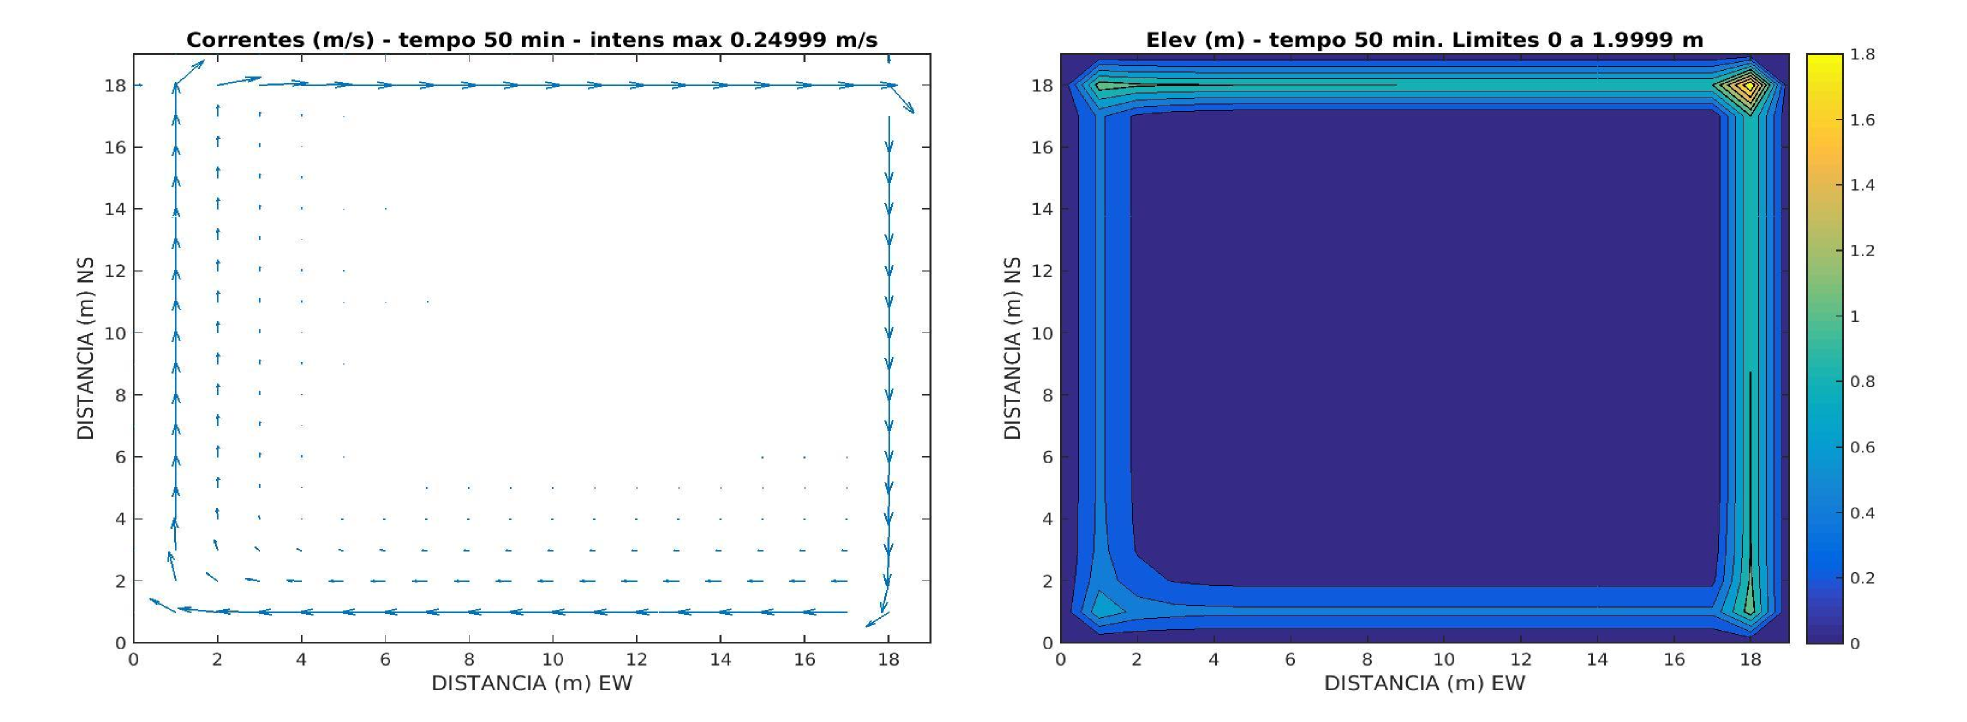
\includegraphics{/home/tparente/danilo/mestrado/github/IOF814/Lista2/outputs/output_report/fig1_1.png}}}
\caption{Fig 1.1 - Campo de correntes (esquerda) e elevação da superfície livre do mar (direita) para o último
 instante de tempo modelado pela função de corrente.}
\label{fig1:1}
\end{figure}

\dotfill

    \subparagraph{Ex2}\label{ex2}

A simulação de um sistema hidrodinâmico 1D foi realizado, utilizando-se
o seguindo conjunto de equações pra águas rasas:

\begin{equation}
    \frac{\partial{v}}{\partial{t}} = - g\frac{\partial{\eta}}{\partial{y}}
    \label{ex2:1}
\end{equation}

\begin{equation}
    \frac{\partial{\eta}}{\partial{t}} = -H\frac{\partial{v}}{\partial{y}}
    \label{ex2:2}
\end{equation}

Assumindo um canal na direção y, simulando o Canal de São Sebastião
(CSB), podemos discretizar (\ref{ex2:1}) e (\ref{ex2:2}), considerando
os efeitos difusivos e decaimento:

\begin{equation}
    \frac{v^{n+1}_{j} - v^{n-1}_{j}}{2\Delta{t}} = -g\bigg[ \frac{\eta^{n}_{j+1}  - \eta^{n}_{j-1}}{2\Delta{y}} \bigg] + D\bigg[ \frac{v^{n}_{j+1} - 2v^{n}_{j} + v^{n}_{j-1}}{\Delta{y^2}} \bigg] - rv^{n}_{j}
    \label{ex2:3}
\end{equation}
\bigskip

Isolando o termo renovado \(v^{n+1}_{j}\), obtemos:

\begin{equation}
    v^{n+1}_{j} = v^{n}_{j} - g\frac{\Delta{t}}{\Delta{y}}(\eta^{n}_{j+1} - \eta^{n}_{j-1}) + 2D\frac{\Delta{t}}{\Delta{y^2}}(v^{n}_{j+1} - 2v^{n}_{j} + v^{n}_{j-1}) - 2rv^{n}_{j}\Delta{t}
    \label{ex2:4}
\end{equation}

\bigskip
Para a equação (\ref{ex2:2}), discretizamos e isolando o termo
\(\eta^{n+1}_{j}\):

\begin{equation}
    \frac{\eta^{n+1}_{j} - \eta^{n-1}_{j}}{2\Delta{t}} = -H\bigg[ \frac{v^{n}_{j+1} - v^{n}_{j}}{\Delta{y}} \bigg] \Rightarrow \eta^{n+1}_{j} = \eta^{n-1}_{j} - 2H\frac{\Delta{t}}{\Delta{y}}(v^{n}_{j+1} - v^{n}_{j})
    \label{ex2:5}
\end{equation}

O código \href{../codes/ex02.m}{ex02.m} modela as equações (\ref{ex2:4})
e (\ref{ex2:5}), obtendo os resultados apresentados abaixo.
\bigskip

No início da simulação (Fig 2.1, esquerda), observamos as condições
de contorno a sul e norte da grade, e o sinal propagando-se para o
interior do canal. Como consequência dessa propagação de sinal de
\(\eta\), há geração de uma corrente negativa nos contornos sul e norte.


\begin{figure}[!ht]
\centering
\centerline{\hbox{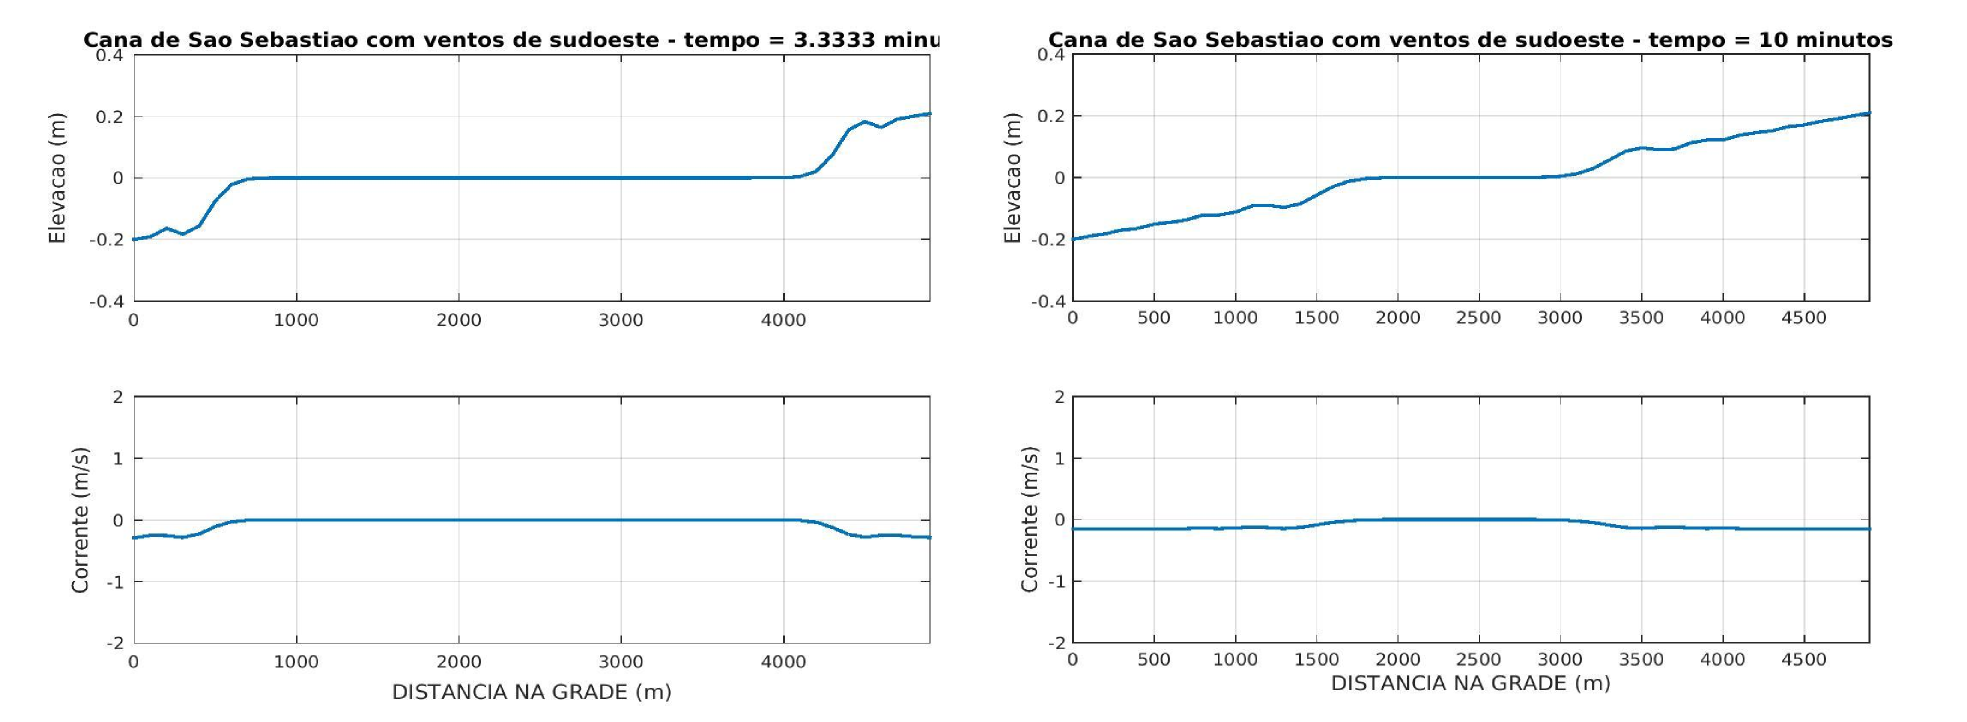
\includegraphics{/home/tparente/danilo/mestrado/github/IOF814/Lista2/outputs/output_report/fig2_1.png}}}
\caption{Fig 2.1 - Elevação da superfície livre do mar (esquerda, superior) e corrente (esquerda, inferior) para o instante
de tempo de 3.4min e para o instante de 10min a direita.}
\label{fig2:1}
\end{figure}

Ambos os sinais convergem para o interior do canal (Figura 2.1, direita)
e, ao se encontrarem, há uma soma destrutiva dos sinais que tende a
equilibrar as oscilações da superfície livre e uma parte deste sinal é
refletida de volta aos contornos (Figura 2.2, esquerda). Desta forma,
com as integrações no tempo, o observado é que a superfície livre entra
em equilíbrio (Figura 2.2, direita).


\begin{figure}[!ht]
\centering
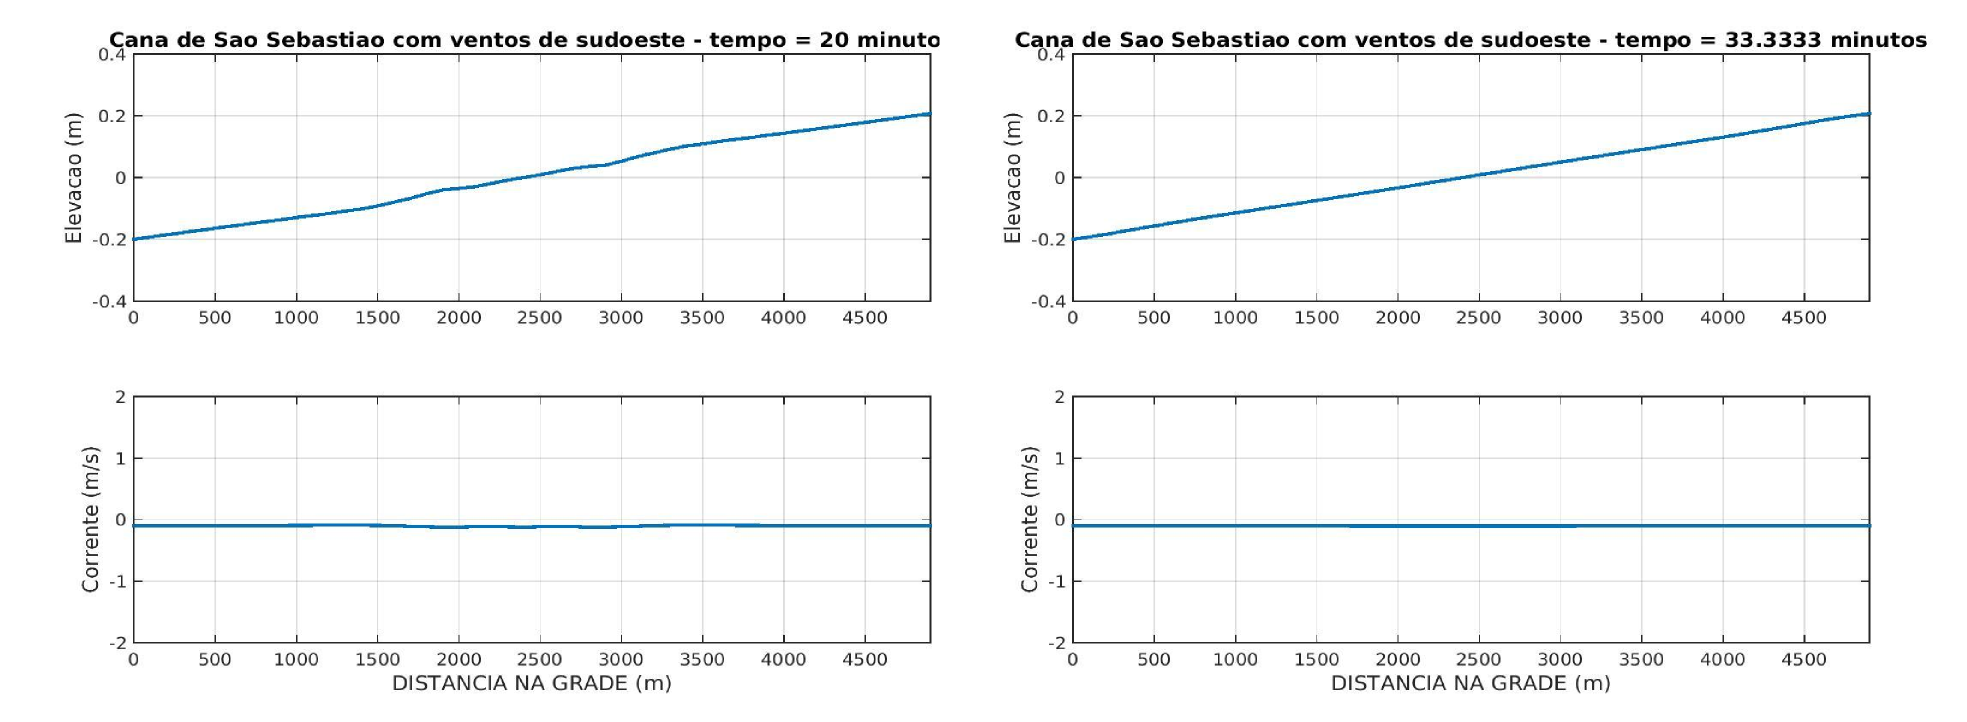
\includegraphics{/home/tparente/danilo/mestrado/github/IOF814/Lista2/outputs/output_report/fig2_2.png}
\caption{Fig 2.2 - Vide Fig2.1, mas para os instantes de tempo de 20min (esquerda) e 32.4min (direita).}
\label{fig2:2}
\end{figure}


\dotfill

    \subparagraph{Ex3 - Parte A}\label{ex3---parte-a}

Considerando as equações:

\begin{equation}
    \frac{\partial{\eta}}{\partial{t}} + H \bigg( \frac{\partial{U}}{\partial{x}} + \frac{\partial{V}}{\partial{y}} \bigg) = 0
    \label{ex3A:eq1}
\end{equation}

\begin{equation}
    \frac{\partial{U}}{\partial{t}} + U\frac{\partial{U}}{\partial{x}} + V\frac{\partial{U}}{\partial{y}} - fV = -g\frac{\partial{\eta}}{\partial{x}} + D_h \bigg( \frac{\partial^2{U}}{\partial{x^2}} + \frac{\partial^2{U}}{\partial{uy^2}} \bigg) - RU
    \label{ex3A:eq2}
\end{equation}

\begin{equation}
    \frac{\partial{V}}{\partial{t}} + U\frac{\partial{V}}{\partial{x}} + V\frac{\partial{V}}{\partial{y}} + fU = -g\frac{\partial{\eta}}{\partial{y}} + D_h \bigg( \frac{\partial^2{V}}{\partial{x^2}} + \frac{\partial^2{V}}{\partial{uy^2}} \bigg) - RV
    \label{ex3A:eq3}
\end{equation}

Uma grade B de Arakawa (Fig.~\ref{ex3A:fig1}), é uma
grade alternada utilizada para modelar as equações hidrodinâmicas 2D,
onde os pontos das componentes de velocidade (u,v) são dados no centro
das células e os pontos de elevação \(\eta\) são definidos nos cantos
das células. Para fins acadêmicos, considera-se, nesta discretização,
um índice para os três pontos (u, v e \(\eta\)).

A discretização das equações \ref{ex3A:eq1}, \ref{ex3A:eq2} e
\ref{ex3A:eq3} segue os seguintes esquemas:

\begin{itemize}
\tightlist
\item
  Esquema explícito, centrado no tempo e no espaço para a
  \textbf{advecção};
\item
  Esquema explícito, avançados no tempo e centrado no espaço para a
  \textbf{difusão} e
\item
  Esquema semi implícito para o \textbf{decaimento}.
\end{itemize}

\begin{figure}[!ht]
\centering
\centerline{\hbox{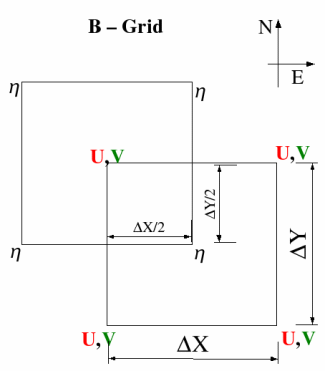
\includegraphics{/home/tparente/danilo/mestrado/github/IOF814/Lista2/outputs/output_report/b-grid.png}}}
\caption{Fig 3.1 - Grade B de Arakawa, com pontos do tipo \(\eta\) localizados nos cantos das células
e pontos do tipo u,v localizados no centro das células. }
\label{ex3A:fig1}
\end{figure}

Ao programar as equações discretizadas, devemos inicialmente calcular as
componentes de velocidade e, então, a aplicar a equação da continuidade.
Desta forma, a discretização será apresentada desta forma, inicialmente
para a componente u, seguida da componente v e, por fim, \(\eta\).

Importante notar que a discretização das equações das componentes de
velocidade ocorrem em um ponto de referência (j+1,k+1), que corresponde
a um ponto de u,v. Já a discretização da equação da continuidade é dada
em um ponto (j,k), por se tratar de um ponto do tipo \(\eta\), conforme
determina o esquema da grade B de Arakawa utilizada.

\textbf{Componente u ou Eq \ref{ex3A:eq2}}

\begin{equation}
\begin{aligned}
\frac{U^{n+1}_{j+1,k+1} - U^{n-1}_{j+1,k+1}}{2\Delta{t}} + umed\bigg( \frac{U^{n}_{j+3,k+1} - U^{n}_{j-1,k+1}}{2\Delta{x}} \bigg) + vmed\bigg( \frac{U^{n}_{j+1,k+3} - U^{n}_{j+1,k-1}}{2\Delta{y}} \bigg) - fV^{n}_{j+1,k+1} = \\
-g\bigg[  \frac{(\eta^{n}_{j+2,k} + \eta^{n}_{j+2,k+2}) -(\eta^{n}_{j,k} + \eta^{n}_{j,k+2} ) }{2\Delta{x}}  \bigg] + \\
+ D_h\bigg[ \bigg( \frac{U^{n-1}_{j+3,k+1} - 2U^{n-1}_{j+1,k+1} + U^{n-1}_{j-1,k+1}}{\Delta{x^2}} \bigg) + \bigg( \frac{U^{n-1}_{j+1,k+3} -2U^{n-1}_{j+1,k+1} + U^{n-1}_{j+1,k-1}}{\Delta{y^2}} \bigg) \bigg] + \\
- R\bigg( \frac{U^{n}_{j+1,k+1} + U^{n+1}_{j+1,k+1}}{2} \bigg)
\label{ex3A:eq4}
\end{aligned}
\end{equation}

\textbf{Componente v ou Eq \ref{ex3A:eq3}}

\begin{equation}
\begin{aligned}
\frac{V^{n+1}_{j+1,k+1} - V^{n-1}_{j+1,k+1}}{2\Delta{t}} + umed\bigg( \frac{V^{n}_{j+3,k+1} - V^{n}_{j-1,k+1}}{2\Delta{x}} \bigg) + vmed\bigg( \frac{V^{n}_{j+1,k+3} - V^{n}_{j+1,k-1}}{2\Delta{y}} \bigg) + fU^{n}_{j+1,k+1} = \\
-g\bigg[ \frac{(\eta^{n}_{j+2,k+2} + \eta^{n}_{j,k+2}) - (\eta^{n}_{j+2,k} + \eta^{n}_{j,k} ) }{2\Delta{y}}  \bigg] + \\
+ D_h\bigg[ \bigg( \frac{V^{n-1}_{j+3,k+1} - 2V^{n-1}_{j+1,k+1} + V^{n-1}_{j-1,k+1}}{\Delta{x^2}} \bigg) + \bigg( \frac{V^{n-1}_{j+1,k+3} -2V^{n-1}_{j+1,k+1} + V^{n-1}_{j+1,k-1}}{\Delta{y^2}} \bigg) \bigg] + \\
- R\bigg( \frac{V^{n}_{j+1,k+1} + V^{n+1}_{j+1,k+1}}{2} \bigg)
\label{ex3A:eq5}
\end{aligned}
\end{equation}

\textbf{Elevação do nível do mar \(\eta\) ou Eq \ref{ex3A:eq1}}

\begin{equation}
\begin{aligned}
\bigg( \frac{\eta^{n+1}_{j,k} - \eta^{n}_{j,k}}{2\Delta{t}} \bigg) +
H\bigg( \frac{U^{n+1}_{j+1,k+1} + U^{n+1}_{j+1,k-1} - U^{n+1}_{j-1,k+1} - U^{n+1}_{j-1,k-1}}{2\Delta{x}} \bigg) + \\
H\bigg( \frac{V^{n+1}_{j+1,k+1} + V^{n+1}_{j-1,k+1} - V^{n+1}_{j+1,k-1} + V^{n+1}_{j-1,k-1}}{2\Delta{y}} \bigg) = 0
\label{ex3A:eq6}
\end{aligned}
\end{equation}
\bigskip

A vantagem, especificamente, da grade B de Arakawa é a facilidade em
representar os termos de Coriolios, embora dificulte, como já
demonstrado, a representação dos termos de gradiente de elevação e
divergente de velocidade.

\subparagraph{Ex3 - Parte B}\label{ex3---parte-b}

Consiste em um modelo de grade variável no tempo, onde a possibilidade
de inundação ou ressecamento dos elementos de grade é uma importante
característica quando modela-se regiões de planícies de maré ou com
baixa declividade do terreno.

Considerando a solução clássica para este tipo de grade, apresentado em
Flather \& Heaps (1975), partimos das equações:

\begin{equation}
    \frac{\partial{U}}{\partial{t}} + U\frac{\partial{U}}{\partial{x}} + V\frac{\partial{U}}{\partial{y}} = -g\frac{\partial{\eta}}{\partial{x}} - \frac{rU\sqrt{U^2 + V^2}}{D}
    \label{ex3B:eq1}
\end{equation}\begin{equation}
    \frac{\partial{V}}{\partial{t}} + U\frac{\partial{V}}{\partial{x}} + V\frac{\partial{V}}{\partial{y}} = -g\frac{\partial{\eta}}{\partial{y}} - \frac{rU\sqrt{U^2 + V^2}}{D}
    \label{ex3B:eq2}
\end{equation}\begin{equation}
    \frac{\partial{\eta}}{\partial{t}} = -\frac{\partial{(DU)}}{\partial{x}} - \frac{\partial{(DV)}}{\partial{y}}
    \label{ex3B:eq3}
\end{equation}

onde:

\(D(x,y,t) = H(x,y) + \eta(x,y,t)\): é a profundidade instantânea, sendo
H a topografia do terreno e \(\eta\) a elevação do nível do mar e
atentando-se ao fato que H é positivo para o oceano e negativo para o
continente e \(\eta\) é positivo para cima e negativo para baixo.

Desta forma, a cada novo nível de tempo, é necessário testar a grade e
seu valores para determinar se haverá inundação ou exposição do fundo.
Este procedimento é realizado através de uma média ponderada entre os
termos de D, onde, para um \textbf{contorno terrestre a oeste da região
modelada}:

\begin{equation}
\begin{cases}
        (j-1) &\mbox{será ponto úmido},  \mbox{se } 0.5(D_{j-1} + D_j) \ge 0
        \\
        (j-1) & \mbox{será ponto seco}, \mbox{se } 0.5(D_{j-1} + D_j) < 0
\end{cases}
\end{equation}
\bigskip

Em caso do ponto (j-1) se tornar um ponto úmido, o valor de elevação e
corrente são extrapolados da região de oceano para as proximidades do
contorno. Desta forma, podemos implementar o seguinte método de
extrapolação para elevação \(\eta\) e corrente:

\begin{equation}
    \bigg( \eta^{n}_{j-1,k} \bigg)_{\text{extrapolado}} = 1\eta^{n}_{j,k} - \eta^{n}_{j+1,k}
    \label{ex3B:eq4}
\end{equation}

\begin{equation}
    \bigg[ \bigg( UD \bigg)^{n}_{j,k} \bigg]_{\text{extrapolado}} = 2(UD)^{n}_{j+1,k} - (UD)^{n}_{j+2,k}
    \label{ex3B:eq5}
\end{equation}
\bigskip

Por fim, aplica-se (\ref{ex3B:eq4}) e (\ref{ex3B:eq5}) para renovar no
tempo as variáveis no ponto (j-1). Um exemplo de aplicação, seria
utilizar as variáveis extrapoladas da seguinte forma:

\begin{equation}
    \eta^{n+1}_{j-1} = \bigg( \eta^{n}_{j-1} \bigg)_{\text{extrapolado}} - \frac{\Delta{t}}{\Delta{x}}\bigg\{ \bigg[ (UD)^{n}_{j} \bigg]_{\text{extrapolado}} -(UD)^{n}_{j-1} \bigg\}
    \label{ex3B:eq6}
\end{equation}
\bigskip

Para um \textbf{contorno terrestre a norte da área modelada}, aplicamos
o mesmo procedimento, onde:

\begin{equation}
\begin{cases}
        (k+1) &\mbox{será ponto úmido},  \mbox{se } 0.5(D_k + D_{k+1}) \ge 0
        \\
        (k+1) & \mbox{será ponto seco}, \mbox{se } 0.5(D_k + D_{k+1}) < 0
\end{cases}
\end{equation}

Obteremos, então, o seguindo par de equações para elevação e corrente:

\begin{equation}
    \bigg( \eta^{n}_{,k+1} \bigg)_{\text{extrapolado}} = 1\eta^{n}_{k+1} - \eta^{n}_k
    \label{ex3B:eq7}
\end{equation}

\begin{equation}
    \bigg[ \bigg( VD \bigg)^{n}_{j,k} \bigg]_{\text{extrapolado}} = 2(VD)^{n}_{j,k-1} - (VD)^{n}_{j,k-2}
    \label{ex3B:eq8}
\end{equation}
\bigskip

Renovando, enfim, a elevação para o contorno terrestre a norte com:

\begin{equation}
    \eta^{n+1}_{j,k+1} = \bigg( \eta^{n}_{j,k+1} \bigg)_{\text{extrapolado}} - \frac{\Delta{t}}{\Delta{y}}\bigg\{ \bigg[ (VD)^{n}_{j,k+1} \bigg]_{\text{extrapolado}} -(VD)^{n}_{j,k} \bigg\}
    \label{ex3B:eq9}
\end{equation}

\dotfill

    \subparagraph{Ex4}\label{ex4}

O método dos mínimos quadrados (Least Square) trata-se um técnica de
interpolação de dados em uma grade a partir de dados conhecidos (in situ
ou saídas de modelos globais). Com isso, conseguimos impor condições
iniciais mais adequadas aos modelos, principalmente em modelos
operacionais, com informações mais próximas da realidade, a fim de obter
resultados mais acurados como produto do modelo.

Trata-se uma técnida conhecida e bem formulada, facilmente resolvida
numericamente por um esquema de sistema linear, conforme programado e
comentado no código \href{../codes/ex04.m}{ex04.m}.

Abaixo são apresentadas as imagens com os os dados originais uma grade
teórica formulada (Figura 4.1, esquerda) e o produto da utilização do
método, preenchendo toda a grade elaborada com dados interpolados a
partir dos pontos conhecidos (Figura 4.1, direita).

A utilização deste método é muito bem conhecida e aplicada em modelos no
mundo todo, onde são implementados modelos com assimilação de dados
(dado in situ ou de satélite) ou aninhamento de grades com modelos
globais. Sua facilidade de implementação e os ganhos em acurácia do
produto modelado são os motivos de sua implementação, uma vez que as
simulações não começarão a partir do repouso, como em modelos
acadêmicos, mas sim a partir de condições que representam o mais próximo
possível da realidade.

Desta forma, ao utilizarmos um modelo devidamente calibrado e validado,
com condições iniciais que representam o estado inicial do sistema,
obteremos produtos cada vez mais representativos ao real.

\begin{figure}[!ht]
\centering
\centerline{\hbox{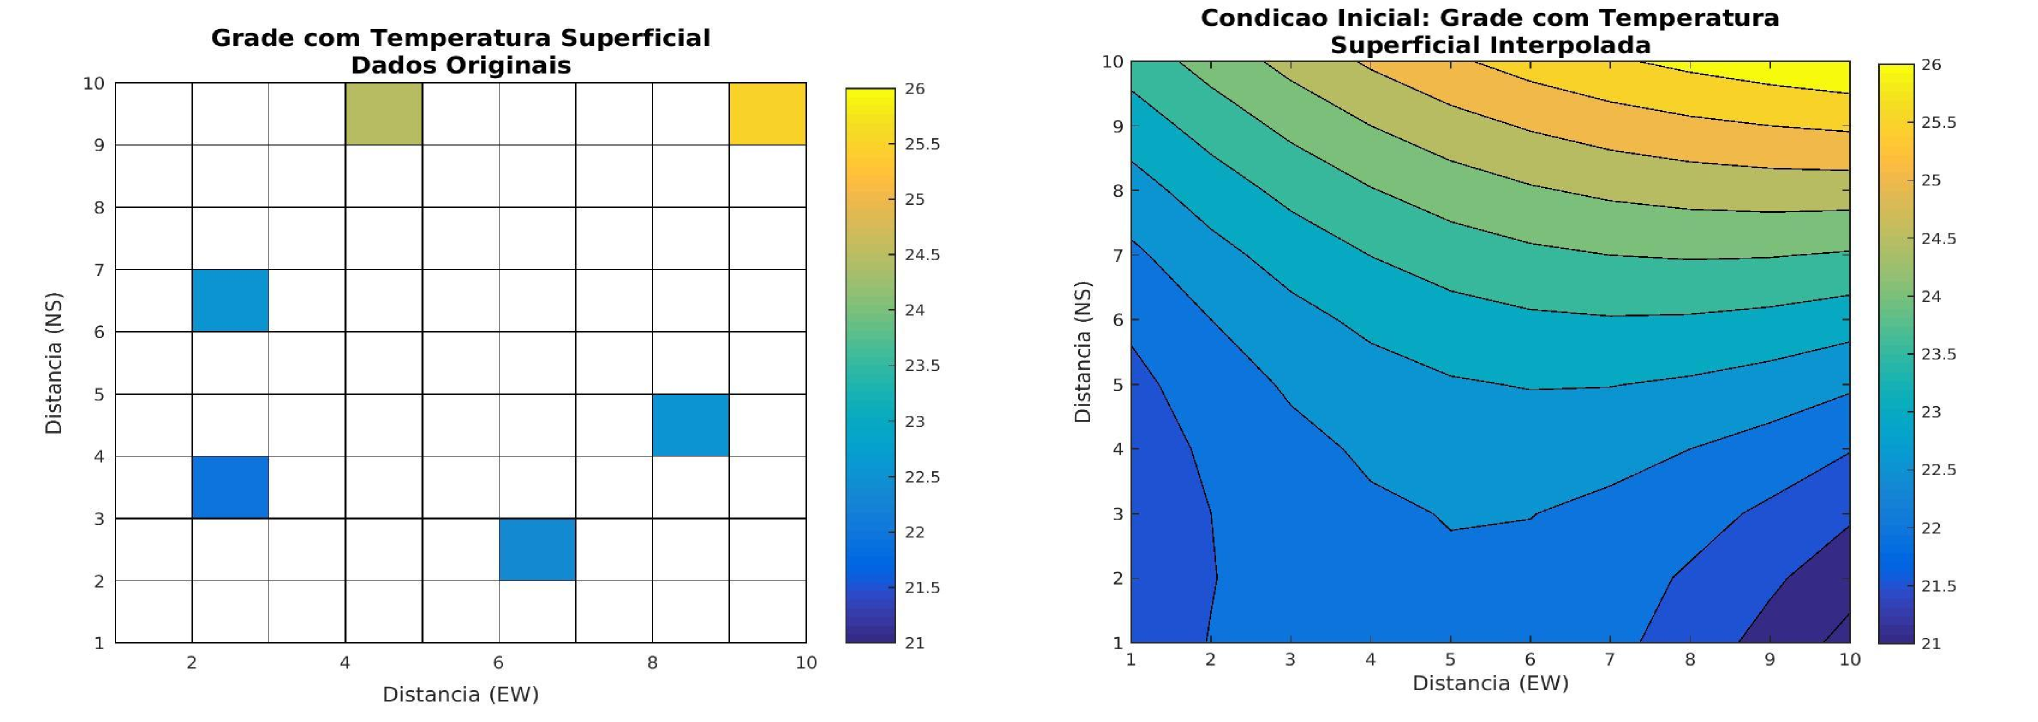
\includegraphics{/home/tparente/danilo/mestrado/github/IOF814/Lista2/outputs/output_report/fig4_1.png}}}
\caption{Fig 4.1 - Grade com dados conhecidos de temperatura (esquerda) e mesma grade com os
dados interpolados pelo Método dos Mínimos Quadrados (direita).}
\label{fig4:1}
\end{figure}

\dotfill

    \subparagraph{Ex5}\label{ex5}

Código do exercício localizado em \href{../codes/ex05.m}{ex05.m} e as
imagens a seguir são um resumo da simulação realizada.

O modelo numérico para a região de Santos foi realizado, utilizando-se
dados batimétricos extraídos do etopo1 (Figura 5.1, esquerda) e um campo de vento
teórico e homogêneo no espaço e tempo (Figura 5.1, direita) de sudoeste.

\begin{figure}[!ht]
\centering
\centerline{\hbox{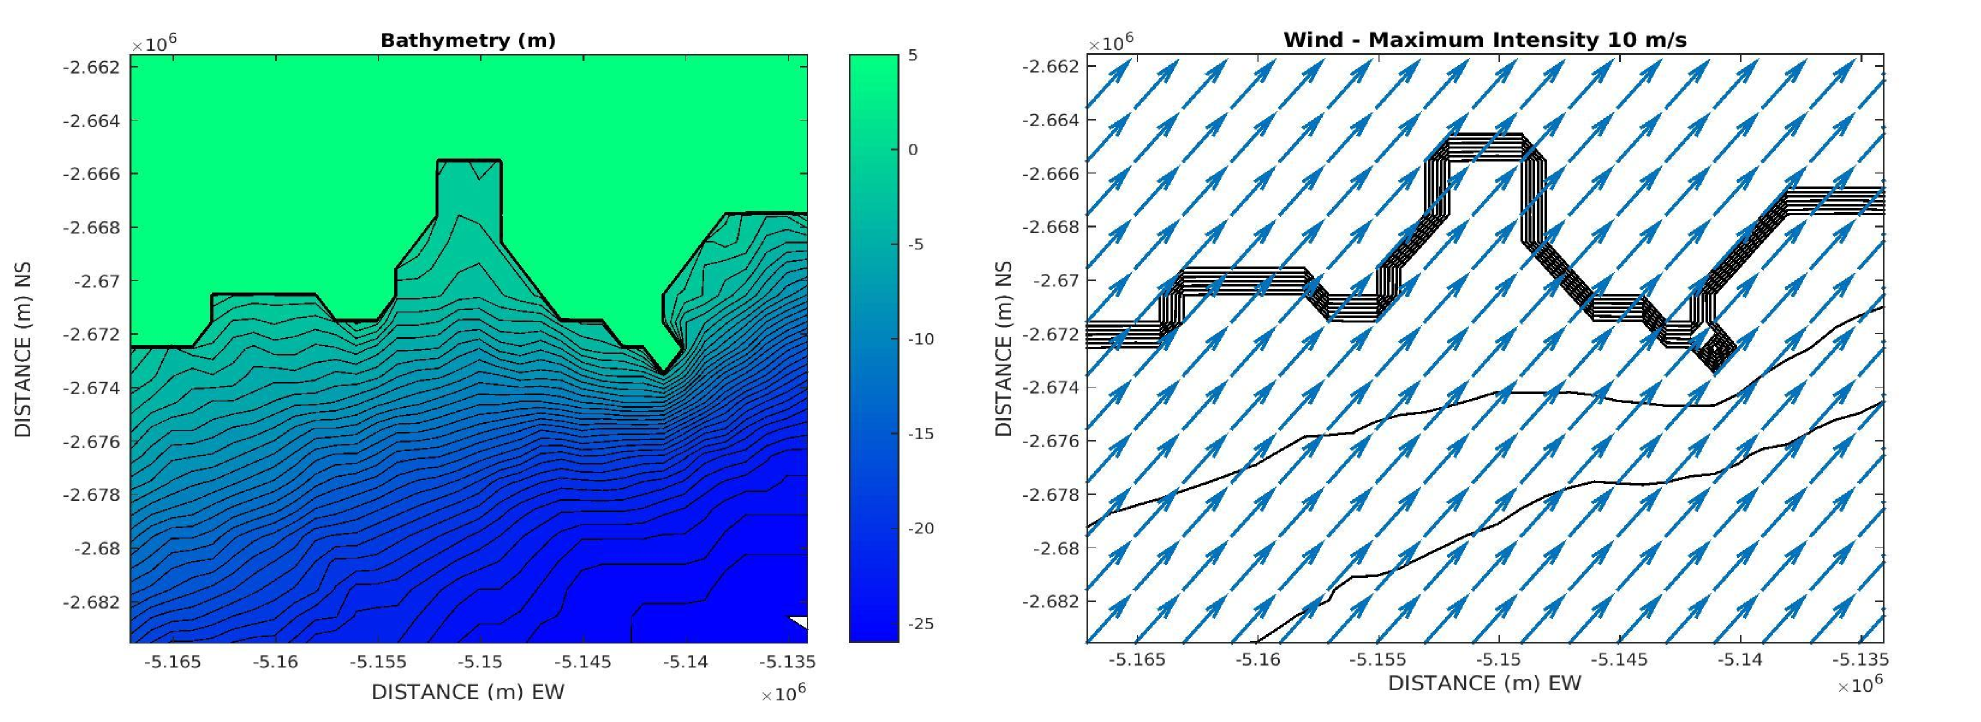
\includegraphics{/home/tparente/danilo/mestrado/github/IOF814/Lista2/outputs/output_report/fig5_1.png}}}
\caption{Fig 5.1 - Batimetria (esquerda) e campo de ventos (direita) utilizados na
simulação deste exercício, compreendo a região de Santos e parte da Plataforma
continental adjacente.}
\label{fig5:1}
\end{figure}

Como resultado da simulação, observamos o campo de corrente gerado pelas
forçantes (vento e elevação nos contornos) na primeira hora modelada
(Figura 5.2) e as oscilações causadas. Nota-se que, as regiões com linha
de costa situada a leste/nordeste há um acúmulo de água, causando uma
sobre elevação da superfície livre associado ao vento de sudoeste e,
para regiões com linha de costa a oeste/sudoeste, observamos um desnível
da superfície livre.

\begin{figure}[!ht]
\centering
\centerline{\hbox{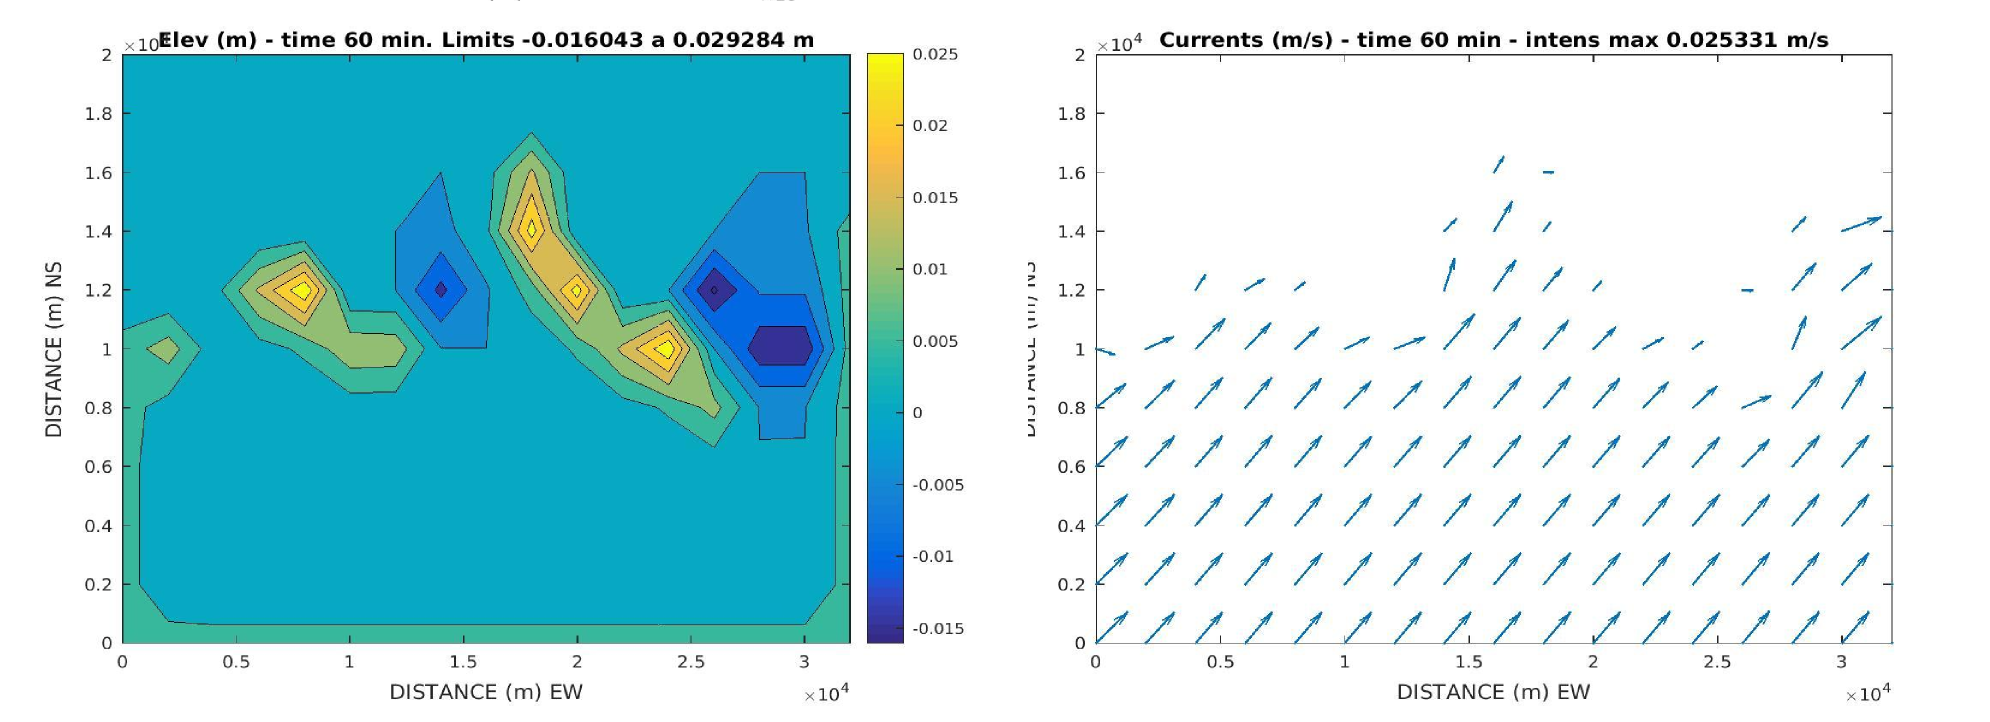
\includegraphics{/home/tparente/danilo/mestrado/github/IOF814/Lista2/outputs/output_report/fig5_2.png}}}
\caption{Fig 5.2 - Campo de elevação da superfície livre do mar (esquerda) e campo de correntes
geradas (direita), para o instante de 60min de simulação.}
\label{fig5:2}
\end{figure}

Para o instante referente a metade do tempo simulado (Figura 5.3),
observamos a propagação do sinal da elevação nos contornos para o
interior da região modelada, onde a única subregião associada a um
desnível da superfície livre situa-se mais leste do domínio,
possivelmente associada, ainda, ao vento homogêneo de sudoeste. Quanto a
circulação, observa-se uma intensificação da corrente a oeste do domínio
com correntes mais fracas próximos aos contorno fechados.

Decorridos toda a simulação, o campo de elevação da superfície livre do
mar (Figura 5.4, esquerda) mostra uma intensificação do cenário já
discutido acima. Nota-se que, a leste do domínio modelado, há um
acentuado desnível, atingindo valores próximos a \(-0.15m\) e, os
maiores valores encontrados, correspondem ao sinal propagado da condição
de contorno estabelecida no modelo, de 0.25m em todos os contornos
abertos. Para o campo de correntes (Figura 5.4, direita), encontramos
máximos valores de \(0.37 m.s^{-1}\), seguindo o mesmo padrão observado
ao longo de toda a simulação, com correntes intensificadas nas regiões
de maior gradiente de elevação do nível do mar.

\begin{figure}[!ht]
\centering
\centerline{\hbox{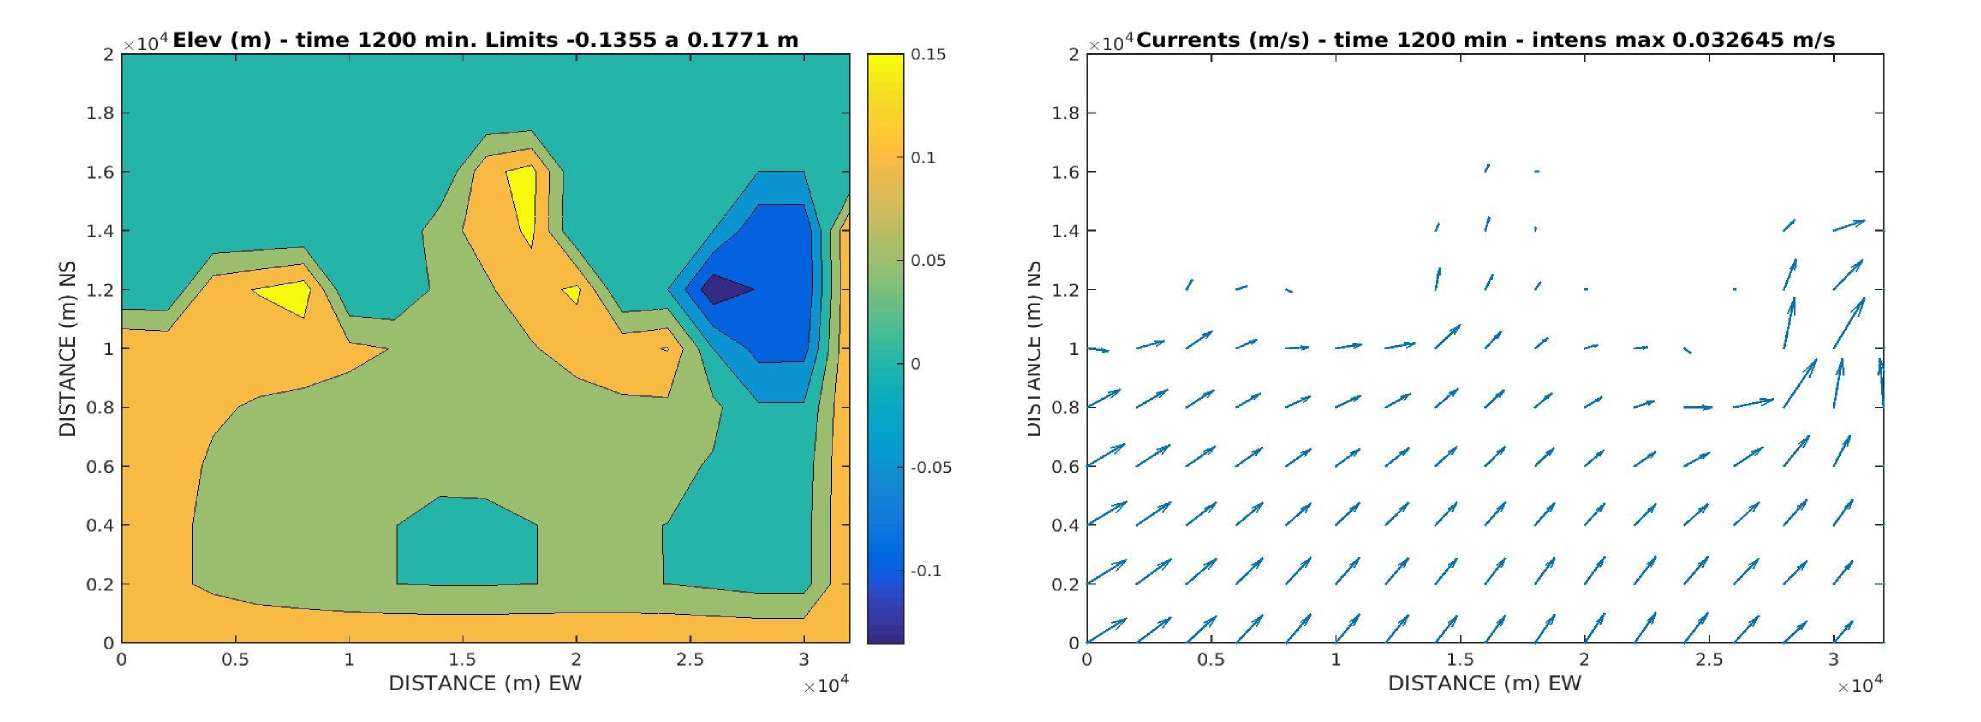
\includegraphics{/home/tparente/danilo/mestrado/github/IOF814/Lista2/outputs/output_report/fig5_3.png}}}
\caption{Fig 5.3 - Vide Fig 5.2, mas para o instante de 1200min.}
\label{fig5:3}
\end{figure}

\bigskip
\begin{figure}[!ht]
\centerline{\hbox{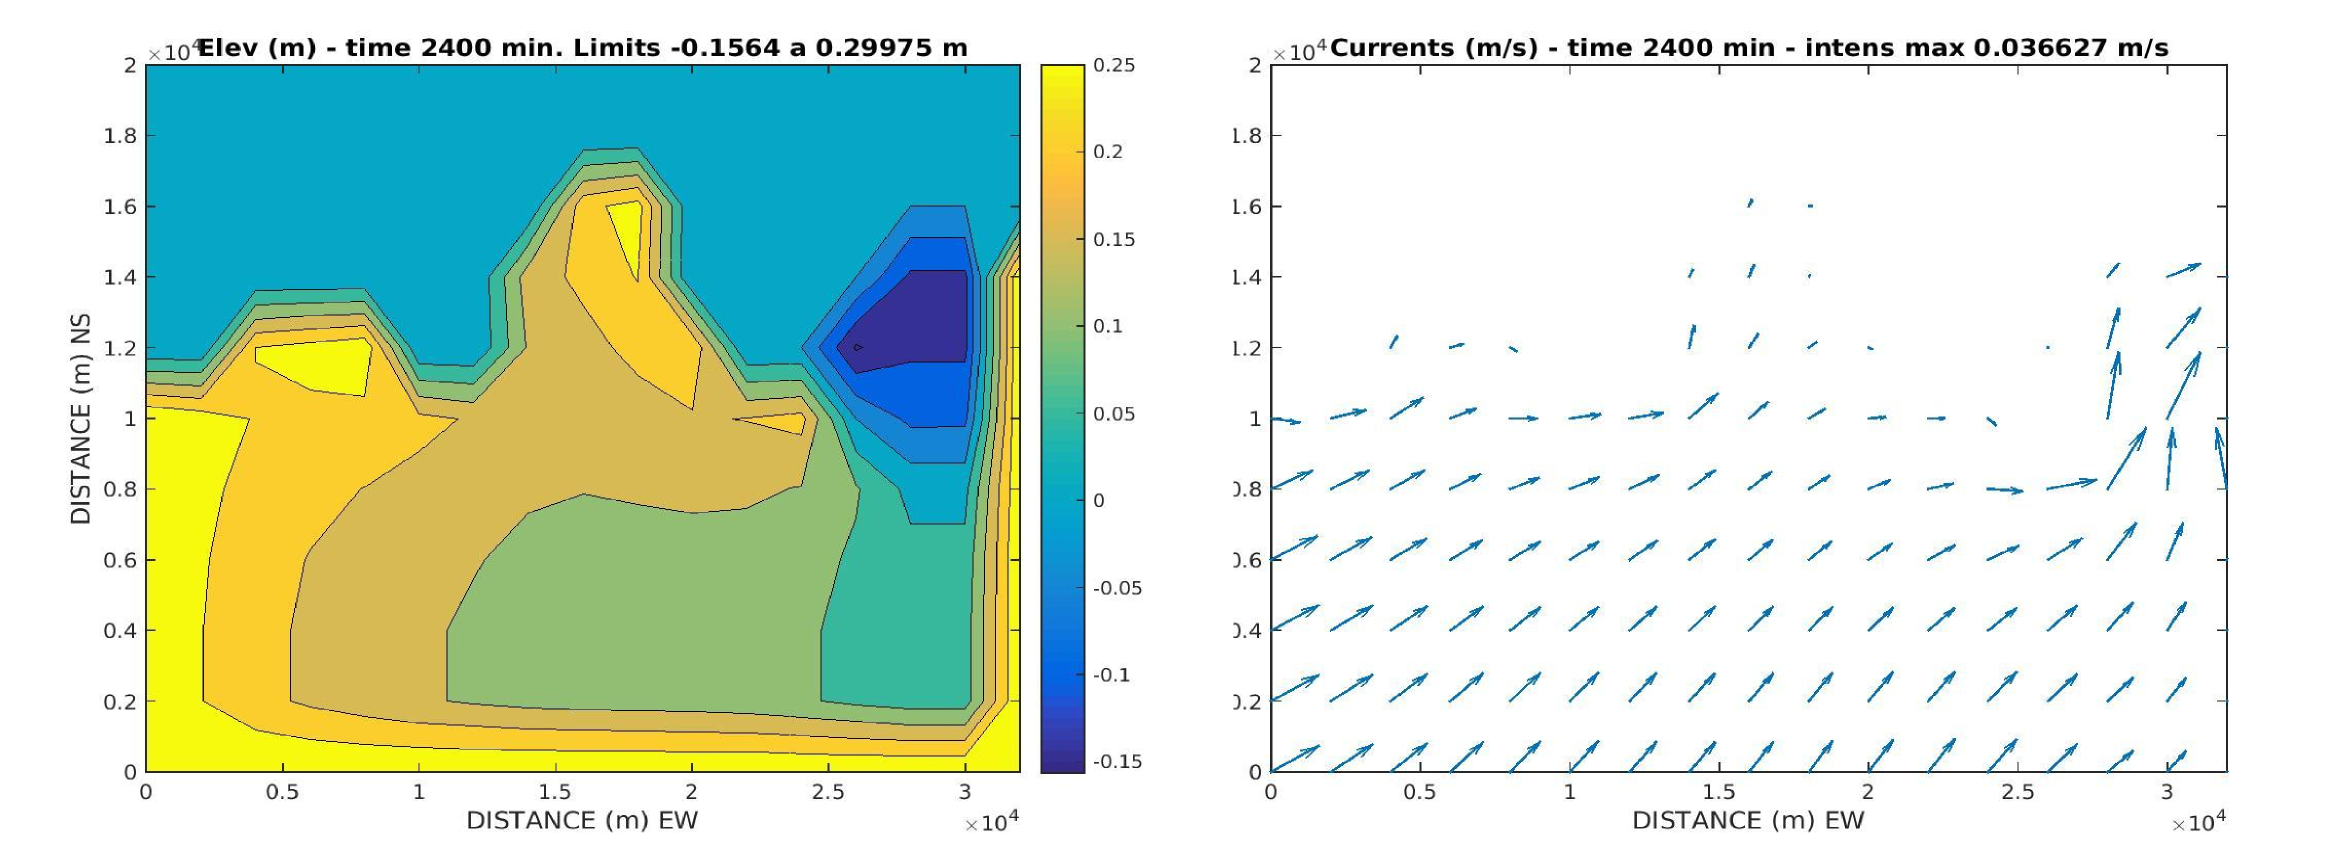
\includegraphics{/home/tparente/danilo/mestrado/github/IOF814/Lista2/outputs/output_report/fig5_4.png}}}
\caption{Fig 5.4 -  Vide Fig 5.2, mas para o instante de 2400 min.}
\label{fig5:4}
\end{figure}
\bigskip


    \end{document}
